% Преамбула

% определяем формат страницы и тип документа ( А4, 12 пунктов, статья)
\documentclass[a4paper,12pt]{article}

% Задаём отступы и межстрочный интервал
\usepackage[top=2cm,bottom=2cm,left=3cm,right=2cm,marginparwidth=1.75cm]{geometry}

% подключаем пакеты расширения LaTeX
\usepackage{cmap}					% поиск в PDF
\usepackage[T2A]{fontenc}			% кодировка
\usepackage[utf8]{inputenc}			% кодировка исходного текста
\usepackage[english,russian]{babel}	% Русский язык и переносы
\usepackage{indentfirst} 			% красная строка
\frenchspacing						
\usepackage[utf8]{inputenc}			% кодировка	
\usepackage[T1]{fontenc}			

% полезные пакетики
\usepackage{amsmath} 									% для продвинутых формул
\usepackage{graphicx}									% для графиков
\usepackage[colorinlistoftodos]{todonotes}				% для пометок
\usepackage[colorlinks=true, allcolors=blue]{hyperref}	% расширенная поддержка гиперссылок
\usepackage{comment}									% многострочные комментарии
\usepackage{ulem}										% зачёркнутый текст
\usepackage{xcolor}										% цветной текст
\usepackage{color}										% цветной код
\usepackage{listings}									% отображает блоки кода

% настройка пакета подсветки исходного кода (не совсем рабочий)
\lstloadlanguages{ [LaTeX ] TeX, bash , Fortran , Perl ,C++,make} 
\lstset{ 			language =[LaTeX ] TeX,		 % выбираем язык по умолчанию
                    extendedchars=true , 		 % включаем не латиницу (не работает)
                    escapechar =| , 			 % |«выпадаем» в LATEX|
                    frame=tb , 					 % рамка сверху и снизу ( lr - слева, справа )
                    commentstyle=\itshape , 	 % шрифт для комментариев
                    stringstyle =\bfseries }	 % шрифт для строк



\author{Андрей Родин} % Вводим своё имя
\title{Отчёт по калибровке магнитометров в ГКВ-11}  % Заголовок
\date{\today} % установка даты

\begin{document}

\maketitle

\begin{abstract}
    Abstract
\end{abstract}

\section{Введение}
\subsection{О погрешностях}
Используемая модель магнитного поля WMM 2015 имеет погрешность определения магнитного склонения, представленную на рисунке ~\ref{fig:WMM_error_field}. Магнитное склонение на широте и долготе Зеленограда равняется $11.24^\circ$ на восток с ошибкой $0.41^\circ$

\begin{figure}[htb] % опция [h] ставит картинку именно в это место,
% не раскидывая рисунки по статье
\centering
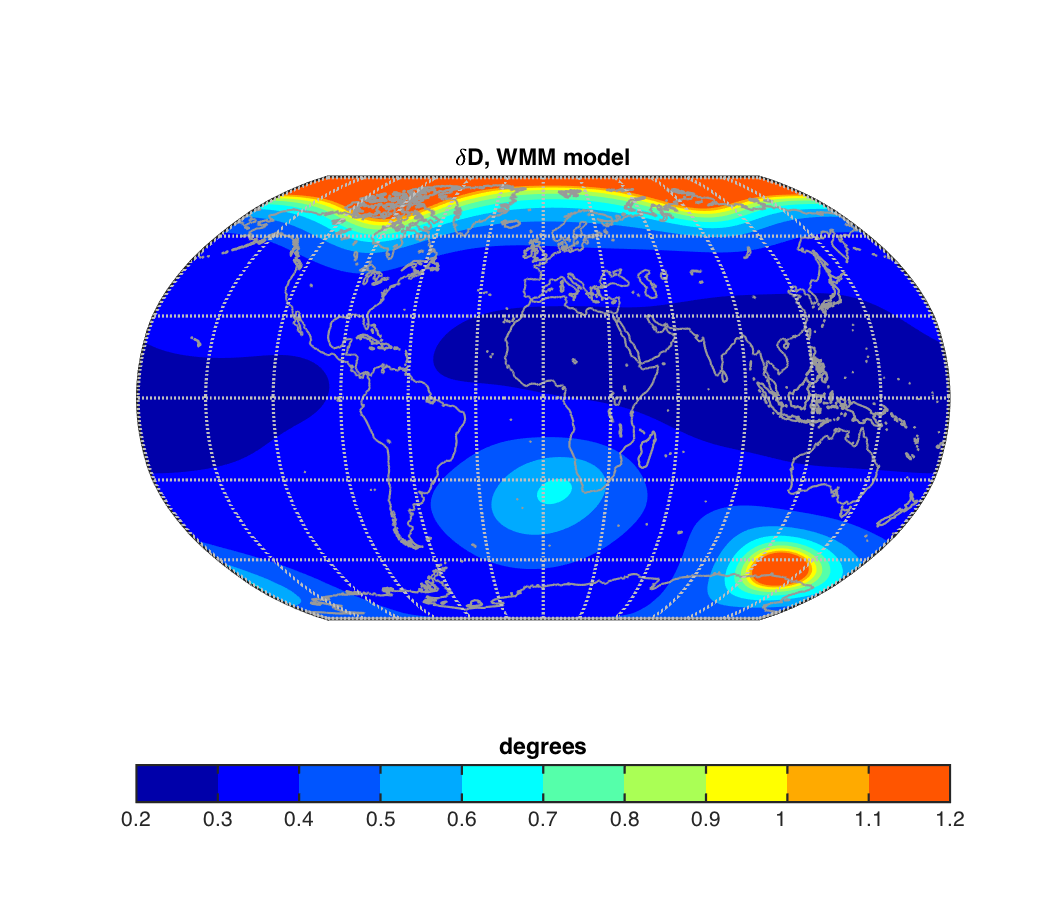
\includegraphics[width=0.75\textwidth]{PICS/WMM2015_Error_Declination.png} % width отвечает за размер картинки
\caption{\label{fig:WMM_error_field} Ошибка склонения WMM2015 без учёта влияния местных аномалий.} % тут же поставили label для возможности ссылаться на рисунок
\end{figure}

В средней полосе России имеем погрешность определения склонения  $0.3-0.5^\circ$
\vspace{\baselineskip}

Погрешность измерения отклонения сданий Миэт от географического севера по картографическим сервисам  $\approx 0.3^\circ$ (По данным карт Яндекс и Google, это направление составляет $13.3^\circ$). Таким образом, методика проверки измерений имеет максимальную погрешность в $0.7^\circ$. 


\section{Методы}
\subsection{Методика проверки калиброванных измерений}
\subsubsection{Калибровка сферы}
При определённом предварительно местном направлении на географический север, прибор ГКВ-11 располагается по направлению севера. После включения прибора и начала работы алгоритма БИНС начинается вестись запись показаний магнитометра и алгоритма БИНС в виде кватерниона. После начала записи прибор вращается во всевозможных направлениях. По завершению вращений ГКВ-11 помещается в исходное положение. Так проводится несколько испытаний. При возвращении в исходную позицию алгоритм БИНС накапливает ошибку курса, поэтому после проведения испытаний отбираются записи экспериментов с наименьшей накопленной ошибкой. Массив кватернионов положения будет представлять эталонные данные для калибровки магнитометра. На широте и долготе Зеленограда вектор магнитной индукции магнитного поля земли входит в землю под углом наклонения  $18.6^\circ$ к вертикали и углом склонения $11.24^\circ$ к направлению на север. Зная эти углы можно  довернуть кватернион положения на соотвевтствующий кватернион поворота, тем самым получив эталонный вектор магнитного поля. 
В итоге, после экспериментов мы имеем два набора данных: массив векторов магнитного поля $M_r$ и массив эталонных векторов предполагаемого магнитного поля $M_e$. Для нахождения матриы исправления <<мягких>>  ошибок $A$ и вектора сдвига $b$, отвечающего за <<жёсткие>>  ошибки, используется метод наименьшик квадратов (МНК):

\[ \left[ M_e - A\left(
M_r - b \right)
\right]^2 \rightarrow min
\]

Один из проведённых экспериментов представлен на рисунке ~\ref{fig:one_of_experiments}.

\begin{figure}[htb] % опция [h] ставит картинку именно в это место,
% не раскидывая рисунки по статье
\centering
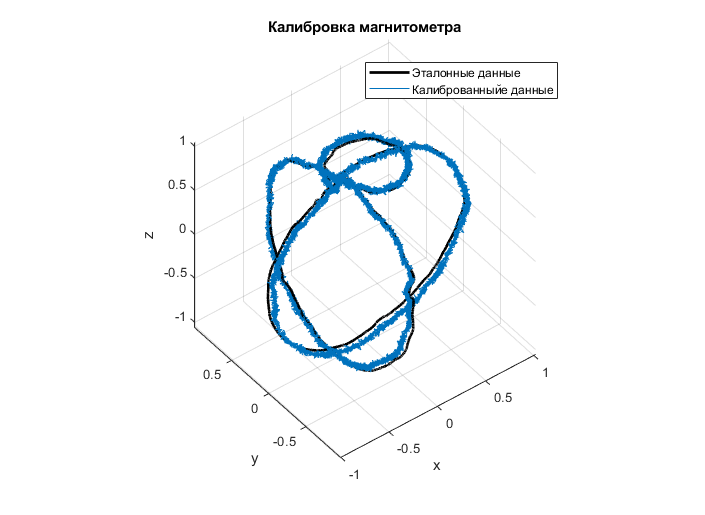
\includegraphics[width=0.8\textwidth]{PICS/one_of_experiments.png} % width отвечает за размер картинки
\caption{\label{fig:one_of_experiments} Вращение ГКВ-11 по трём осям последовательно.} % тут же поставили label для возможности ссылаться на рисунок
\end{figure}

\subsubsection{Калибровка кольца}
В большинстве прикладных задач нет возможности вращать датчик во всевозможных направлениях перед началом работы. Но практически всегда есть возможность вращать датчик на $360^\circ$ вокруг какой-либо из осей. Помимо калибровки сферических данных дополнительно была рассмотрена калибровка по выражденным данным - по кольцу. Алгоритм калибровки не отличается от алгоритма предыдущего пункта, при этом вдоль одной из осей (вырожденной) происходит неверное масштабирования калибровочной матрицы, что не повлияет на погрешность вычислений в плоскости кольца.

\subsubsection{Измерения откалиброванным прибором}
После проведения калибровки ГКВ-11 располагается в случайном горизонтальном положении с последующим  считыванием вектора магнитного поля. При этом было проведено два вида измерений: с выключением-включением ГКВ-11 для каждого измерения угла и с бесперебойной подачей питания.

Проекции измеренных и откалиброванных точек на плоскость XY для различных углов показаны на рисунке ~\ref{fig:round_circle}.
\begin{figure}[htb] % опция [h] ставит картинку именно в это место,
% не раскидывая рисунки по статье
\centering
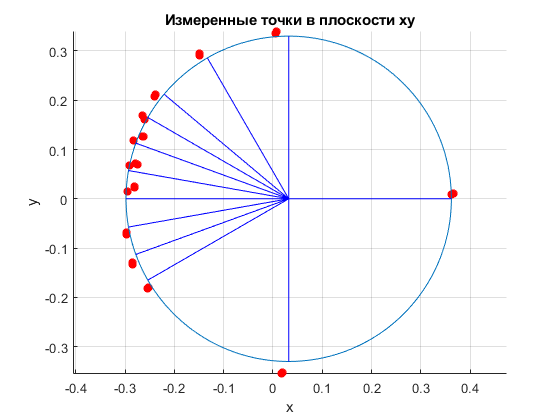
\includegraphics[width=0.7\textwidth]{PICS/measdots.png} % width отвечает за размер картинки
\caption{\label{fig:round_circle} Измеренные точки магнитометра при различных углах с выключением питания.} % тут же поставили label для возможности ссылаться на рисунок
\end{figure}

По измеренным данным был постоен график ошибок определения направления на магнитный север, представленный на рисунке ~\ref{fig:errs1}. 

\begin{figure}[htb] % опция [h] ставит картинку именно в это место,
% не раскидывая рисунки по статье
\centering
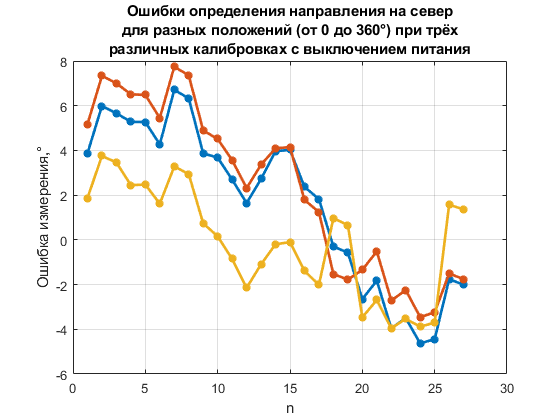
\includegraphics[width=0.7\textwidth]{PICS/magn_out_errors5.png} % width отвечает за размер картинки
\caption{\label{fig:errs1}Погрешности определения севера в поле с выключением питания.} % тут же поставили label для возможности ссылаться на рисунок
\end{figure}

Был также проведён аналогичный эксперимент но с постоянно включенным питанием ГКВ. Это дало немного лучшие результаты.

При проведении идентичных испытаний с исскуственными помехами - закреплённым магнитом рядом с ГКВ - модуль вектора магнитной индукции увеличился в 1.3 раза, а точность измерений направлений ухудшилась, что показывает рисунок ~\ref{fig:errs2}.

\begin{figure}[htb] % опция [h] ставит картинку именно в это место,
% не раскидывая рисунки по статье
\centering
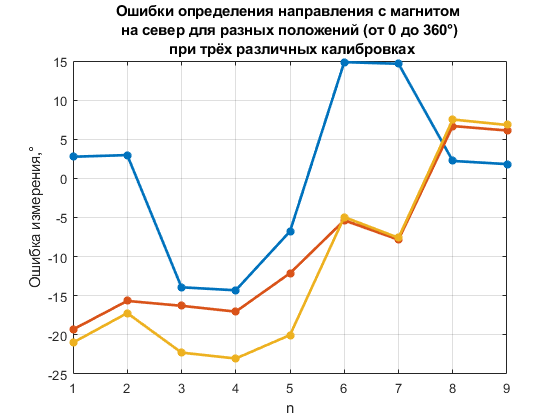
\includegraphics[width=0.7\textwidth]{PICS/outs_magnet_disturb_error2.png} % width отвечает за размер картинки
\caption{\label{fig:errs2}Погрешности определения севера с исскуственной помехой - магнитом.} % тут же поставили label для возможности ссылаться на рисунок
\end{figure}

\section{Результаты}
Абсолютные погрешности определения направления на север в градусах представлены в таблице ~\ref{tab:widgets}. .

\begin{table}[h]
\centering
\begin{tabular}{|l|c|r|}
Измерения & Без помех & С помехами в виде магнита \\\hline
С выключением питания &  $\pm 5^\circ$ & -- \\
С постоянной подачей питания & $\pm 3^\circ$  & $\pm 15^\circ$ \\
\end{tabular}
\caption{\label{tab:widgets}Результаты.}
\end{table}
%Для нахождения калибровочных матриц стенд вращают во всевозможных направлениях, одновременно снимая показания магнитометра и  алгоритма БИНС, выдающего положение в виде кватерниона. 
\end{document}
